\documentclass[a4paper,10pt]{article}

%%%% PRATIQUE POUR LES ALINEAS CHIANTS
\usepackage{indentfirst}

%%%% POUR L'OPTION LABEL= %%%
\usepackage{enumitem}

\setlength{\parindent}{30pt}
\setlength{\parskip}{1ex}
\setlength{\textwidth}{15cm}
\setlength{\textheight}{24cm}
\setlength{\oddsidemargin}{0.2cm}
\setlength{\evensidemargin}{-.7cm}
\setlength{\topmargin}{-.5in}

\usepackage{graphicx}
\usepackage{titling}
\usepackage{listings}
\lstset{%
  basicstyle=\scriptsize\sffamily,%
  commentstyle=\footnotesize\ttfamily,%
  frameround=trBL,
  frame=single,
  breaklines=true,
  showstringspaces=false,
  numbers=left,
  numberstyle=\tiny,
  numbersep=10pt,
  keywordstyle=\bf
}
\newcommand{\subtitle}[1]{%
  \posttitle{%
    \par\end{center}
    \begin{center}\large#1\end{center}
    \vskip0.5em}%
}
\title{\textbf{Inputs/Outputs Scheduling}}
\subtitle{M1 MoSIG : Operating Systems}
\author{Poupin Pierre \and Rouby Thomas}
\date{26/11/2014}

\begin{document}
\maketitle

\section{Introduction, hard drives technology}

Algorithms for I/Os scheduling in use today are motivated by mechanical hard drives technology.
A mechanical hard drive is made :
\begin{itemize}
  \item platters (rotating) on which data is stored.
  \item arm to move r/w heads.
  \item r/w head at the end of the arm.
\end{itemize}

\begin{figure}[h!]
  \begin{center}
    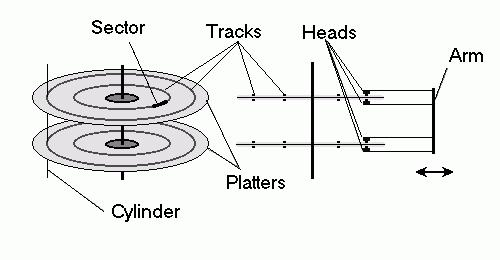
\includegraphics{hard_drive_picture.jpg}
  \end{center}
\end{figure}

%place hard drive picture here
To perform an access to a specific sector :
\begin{itemize}
  \item move the arm to the proper track
  $=>$ takes time: depends on the engine moving the arm.
  \item wait for the desired sector
   $=>$ takes time: depends on the rotating speed of the platters.
  \item select the head and read or write
  $=>$ fast.
\end{itemize}

As a result, the access time to some sector will be :
\begin{itemize}
  \item fast: if the arm is already on the right track and the sector already under the r/w head. (about 125 MB/s $=>$ 500 nanoseconds to get 4 bytes).
  It is the bandwidth of sequential accesses.
  \item slow: otherwise (about 10 ms to get 4 bytes : there is a 20 000 factor).
  It is the latency of a random access.
  
\end{itemize}

Usually, sequential accesses can reach full bandwidth with a small degradation on track change.
Latency is given on average, the exact latency depends on the istance of the arm from the track and on the sector position.

\section{I/Os scheduling}

The CPU is much faster than a hard disk, even at full bandwidth

\end{document}
